\chapter{Desenvolvemento da solución}
\label{chap:desenvolvemento-solucion}

Neste capítulo descríbense os aspectos técnicos da solución desenvolvida, detallando as decisións de
implementación adoptadas en cada etapa do sistema. En particular, abórdase o preprocesado dos datos,
a detección das algas nas imaxes, a normalización das mostras, a arquitectura e o adestramento do
modelo de inferencia e a integración final de todo o fluxo nun programa informático.

\section{Preprocesado de datos}
O primeiro paso da solución consistiu en depurar o \textit{dataset} inicial para reducir a
variabilidade introducida por erros ou inconsistencias básicas nos datos. Para iso desenvolveuse un
\textit{script} en Python, denominado \texttt{01\_script\_filtro.py}, orientado a simplificar o
ficheiro de etiquetas, validar o formato das variables de interese e eliminar imaxes que non puidesen
ser empregadas nas etapas posteriores do pipeline. Ademais da execución deste \textit{script},
realizouse unha revisión posterior adicional baseada en criterios proporcionados polos expertos.

\subsection{\textit{Script} de limpeza}
\subsubsection{Entrada}
O \textit{script} parte de dúas fontes de datos definidas previamente no proxecto:
\begin{itemize}
    \item O ficheiro Excel orixinal proporcionado polos expertos, no que se almacenaban as etiquetas asociadas ás mostras.
    \item A carpeta coas imaxes correspondentes ao \textit{dataset}.
\end{itemize}
De maneira opcional, o programa admite o argumento \texttt{--dry-run}, que permite simular a
limpeza das imaxes sen realizar modificacións sobre os ficheiros.

\subsubsection{Procesado}
En primeiro lugar, compróbase a existencia do ficheiro Excel e procédese á súa lectura mediante
\texttt{pandas}. Unha vez cargado, selecciónanse unicamente as tres columnas relevantes para o
problema abordado: \texttt{Photo\_cod}, \texttt{HPI} e \texttt{IVR}. Esta redución permitiu
traballar só cos metadatos estritamente necesarios para a tarefa de inferencia.

Posteriormente, as variables \texttt{HPI} e \texttt{IVR} convértense a formato numérico. As filas
nas que algunha destas etiquetas non puido interpretarse correctamente elimínanse do conxunto de
datos. Ademais, verificouse que ambos os dous valores fosen enteiros, xa que representan niveis
ordinais e, polo tanto, non tería sentido manter rexistros con valores decimais.

Como parte final desta etapa, revisouse a carpeta de imaxes para detectar ficheiros sen referencia
válida no ficheiro das táboas. As imaxes cuxo identificador non aparecía en \texttt{Photo\_cod}
elimináronse, posto que non podían utilizarse no adestramento nin na avaliación do modelo.

\subsubsection{Saída}
Como resultado, xeráronse dous ficheiros de saída, en formato CSV e Excel, contendo exclusivamente
as columnas \texttt{Photo\_cod}, \texttt{HPI} e \texttt{IVR}. Esta etapa garantiu que as imaxes
conservadas no repositorio dispoñían dunha referencia válida no ficheiro de etiquetas. Cómpre
indicar, porén, que esta comprobación só se aplicou nese sentido. Non se eliminaban automaticamente
as filas do ficheiro de táboas cuxa imaxe asociada non estivese presente na carpeta. Esta limitación
foi tida en conta durante a análise e retómase nas conclusións como posible mellora do pipeline.

\subsection{Resultado da execución}
Tras executar o \textit{script} sobre o \textit{dataset} inicial, composto por 5490 filas no
ficheiro Excel e 4984 imaxes, obtívose o seguinte resultado:
\begin{itemize}
    \item Elimináronse 4 filas con valores non numéricos en \texttt{HPI} ou \texttt{IVR} (por exemplo, \texttt{o}, \texttt{O} ou \texttt{NaN}).
    \item Elimináronse 7 imaxes por non teren correspondencia válida no ficheiro tabular.
\end{itemize}

\subsection{Poda posterior e conclusión}
Despois desta limpeza inicial, aplicouse unha poda adicional para asegurar o cumprimento das regras
de etiquetado establecidas polos expertos. Esta revisión permitiu detectar 4 casos que incumprían
ditos criterios, descritos na
Sección-\ref{sec:descricion-variables-obxectivo}, polo que foron eliminados tanto do conxunto de
imaxes coma dos ficheiros finais de etiquetas.

En conxunto, esta fase de preprocesado permitiu partir dun conxunto de datos máis consistente e
axeitado para o resto do traballo. Aínda que o volume de rexistros descartados non foi elevado, a
limpeza resultou necesaria para evitar que erros de formato ou mostras sen utilidade condicionasen
as etapas posteriores de detección, normalización e inferencia. Tras esta etapa, o conxunto final
quedou composto por 4977 imaxes e 5486 rexistros tabulares.

\textcolor{red}{\textbf{TODO: Engadir nas conclusións que non se borraron as filas no csv que non tiñan referencia a imaxes, pero esto non tivo un impacto real 
en ningunha execución, só sería por perfeccionismo. Ademási comentar que inicialmente non se trataron as imaxes con HPI=0 e IVR=0 (1369)}}

\section{Detección de alga en imaxes}

\subsection{Primeira Aproximación}
Inicialmente procurouse unha solución baseada en técnicas clásicas de visión por computador
empregando a libraría \texttt{OpenCV} para Python en dous script novos, 
\texttt{02\_recortar\_algas.py} e \texttt{02\_debug\_recortar\_algas.py}. O obxectivo era resolver a detección da alga cun
enfoque relativamente simple e lixeiro, evitando nun primeiro momento o uso de modelos de
aprendizaxe profunda. As distintas implementacións probadas compartían unha mesma idea central:
aproveitar os contornos e as características visuais dos obxectos presentes na imaxe para identificar
a alga de interese.

Esta primeira proposta partía de que as fotografías compartían un fondo maioritariamente branco, polo
que, en principio, parecía factible segmentar os distintos elementos da escena mediante técnicas
clásicas. Comezouse empregando o detector de bordes de Canny, un método que resalta cambios bruscos
de intensidade na imaxe e permite identificar posibles contornos. A partir destes contornos
tentouse localizar a alga combinando información sobre cor, posición e forma. Entre outros recursos,
probase a detección dos números identificadores mediante filtrado por cor e a selección dos contornos
cuxa aparencia se aproximaba máis á cor das algas, estimada previamente mediante inspección manual.

A primeira implementación ofreceu resultados moi limitados debido á elevada variabilidade do
\textit{dataset}. En moitos casos detectábanse regras como se fosen algas, especialmente cando eran
pequenas; a cor da alga variaba notablemente en función da iluminación; e os números identificadores
non sempre aparecían na mesma cor, o que impedía a súa eliminación mediante regras sinxelas. En
conxunto, estes factores facían que o algoritmo resultase pouco robusto.

Co fin de mellorar esta primeira aproximación, introducíronse diversos parches orientados a eliminar
elementos alleos á alga. No caso das regras, probouse primeiro a detección de contornos cunha
relación de aspecto semellante á dunha regra e, posteriormente, o uso da transformada de Hough para
detectar liñas rectas que permitisen identificalas. Aínda así, este procedemento seguía fallando con
frecuencia, xa que a regra non sempre aparecía representada como un único contorno claro. Tamén se
intentou eliminar contornos próximos ás liñas detectadas, pero isto provocaba a supresión de partes
da propia alga cando ambas rexións estaban moi próximas na imaxe.

Para os números identificadores empregáronse filtros de cor con distintas configuracións, pero comprobouse
que a súa eficacia era reducida, sobre todo no caso do verde, que se confundía con
facilidade coas tonalidades da alga. Tamén se probou a eliminación destas marcas a partir do tamaño
da súa \textit{bounding box}, pero esta estratexia descartaba igualmente algas pequenas.

Outra hipótese considerada foi asumir que a alga correspondía ao contorno máis centrado da imaxe. Con
todo, esta condición tampouco se cumpría de forma suficientemente consistente, polo que a idea foi
descartada. Así mesmo, experimentouse con técnicas baseadas en histogramas e segmentación automática,
como o método de Otsu, que selecciona automaticamente un valor de corte para separar rexións de
distinta intensidade. Isto tampouco produciu unha separación fiable entre a alga e o resto de
elementos da escena.

Finalmente, tamén se intentou caracterizar unha suposta ``forma de alga'' a partir de medidas como a
compacidade ou a estrutura do contorno. Esta aproximación resultou pouco útil debido á gran
variabilidade morfolóxica presente nas mostras.

As distintas ideas anteriores chegaron a combinarse nun sistema de puntuación ou ``confianza'', no
que cada contorno recibía unha valoración positiva ou negativa segundo a súa semellanza coa alga de
interese. Porén, esta combinación incrementou notablemente a complexidade do código sen mellorar de
maneira suficiente a robustez do método.

Como conclusión, esta primeira aproximación acabou xerando unha implementación relativamente extensa,
de arredor de 500 liñas, e aínda así non ofreceu resultados satisfactorios. Aínda que nesta fase non
se definiron métricas formais, xa que a validación se realizaba manualmente, estimouse que só arredor
do 40\,\% do \textit{dataset} se detectaba de maneira correcta. Algúns exemplos destes recortes
erróneos móstranse na Figura-\ref{fig:recortes-erroneos}. Á vista destes resultados, decidiuse
abandonar este enfoque e optar por unha técnica menos sensible á variabilidade das imaxes, baseada en
detección automática mediante aprendizaxe profunda.

\begin{figure}[htbp]
    \centering
    \begin{subfigure}[t]{0.42\textwidth}
        \centering
        \includegraphics[width=\linewidth]{imaxes/mal_recorte_1.jpg}
        \caption{Alga mal recortada por ter contacto cos bordes.}
    \end{subfigure}
    \hfill
    \begin{subfigure}[t]{0.42\textwidth}
        \centering
        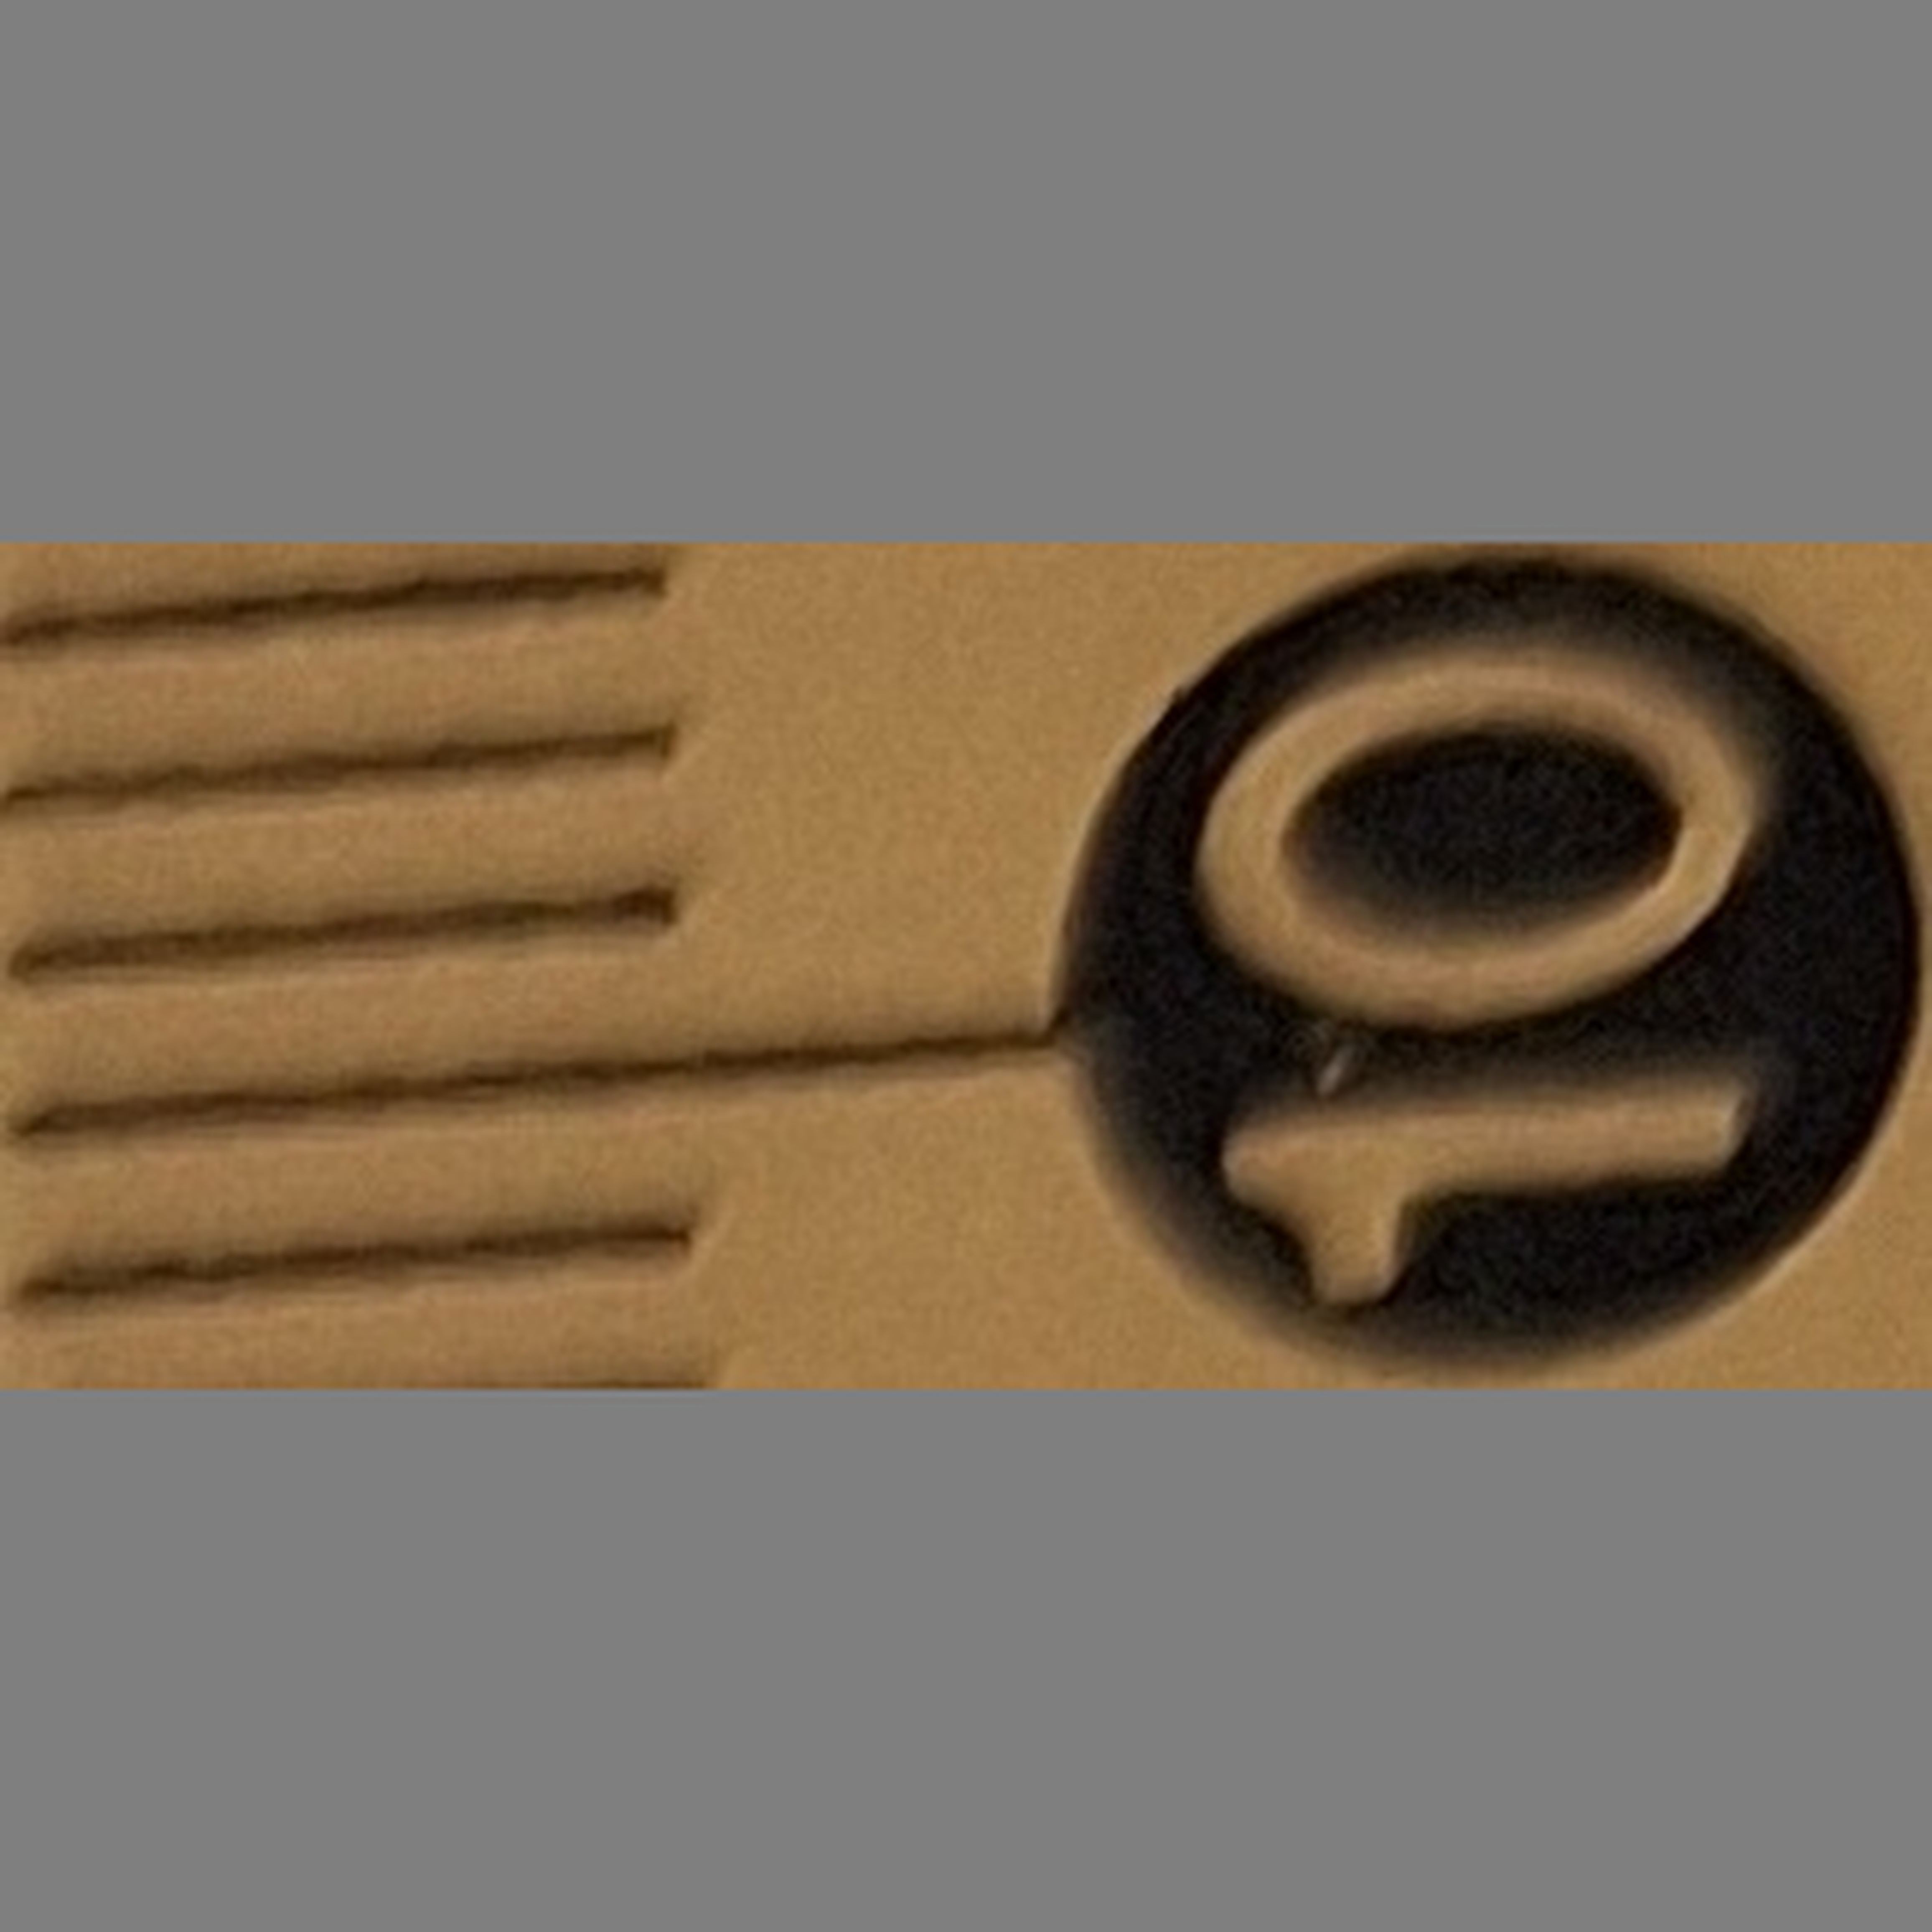
\includegraphics[width=\linewidth]{imaxes/mal_recorte_2.jpg}
        \caption{Números da regra recortados como alga.}
    \end{subfigure}

    \vspace{0.15em}

    \begin{subfigure}[t]{0.42\textwidth}
        \centering
        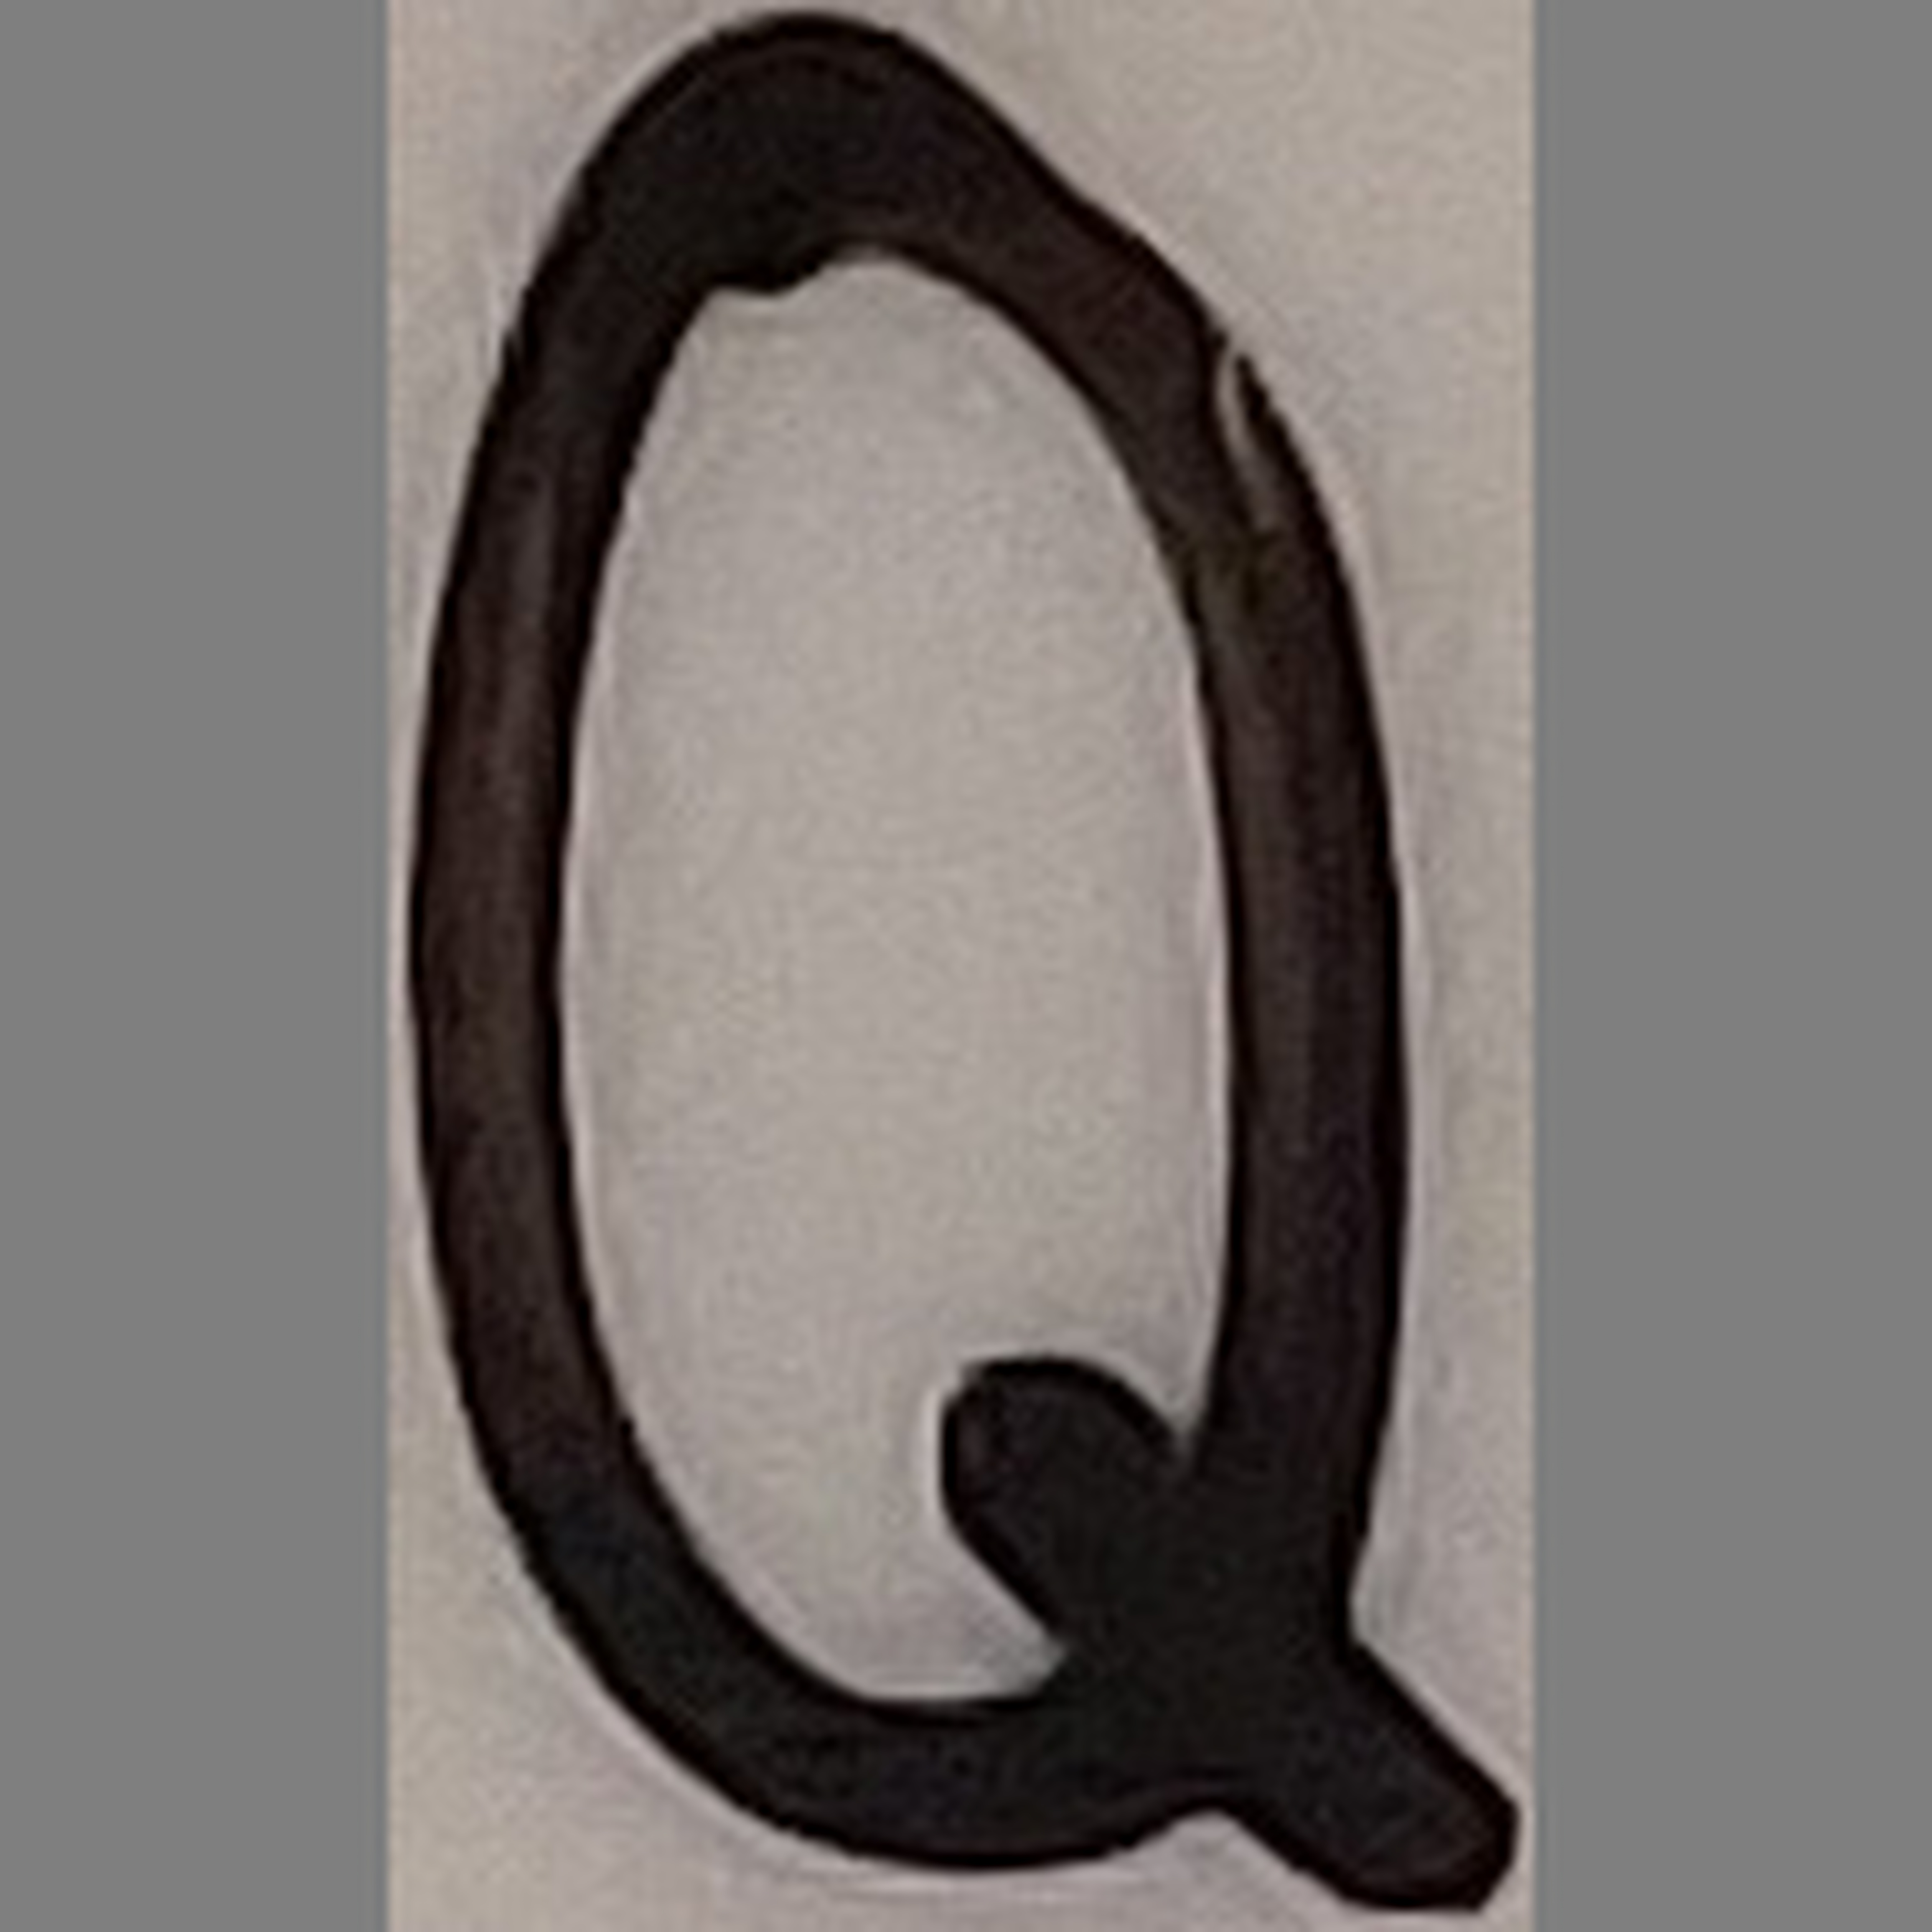
\includegraphics[width=\linewidth]{imaxes/mal_recorte_3.jpg}
        \caption{Letra negra recortada como alga.}
    \end{subfigure}
    \hfill
    \begin{subfigure}[t]{0.42\textwidth}
        \centering
        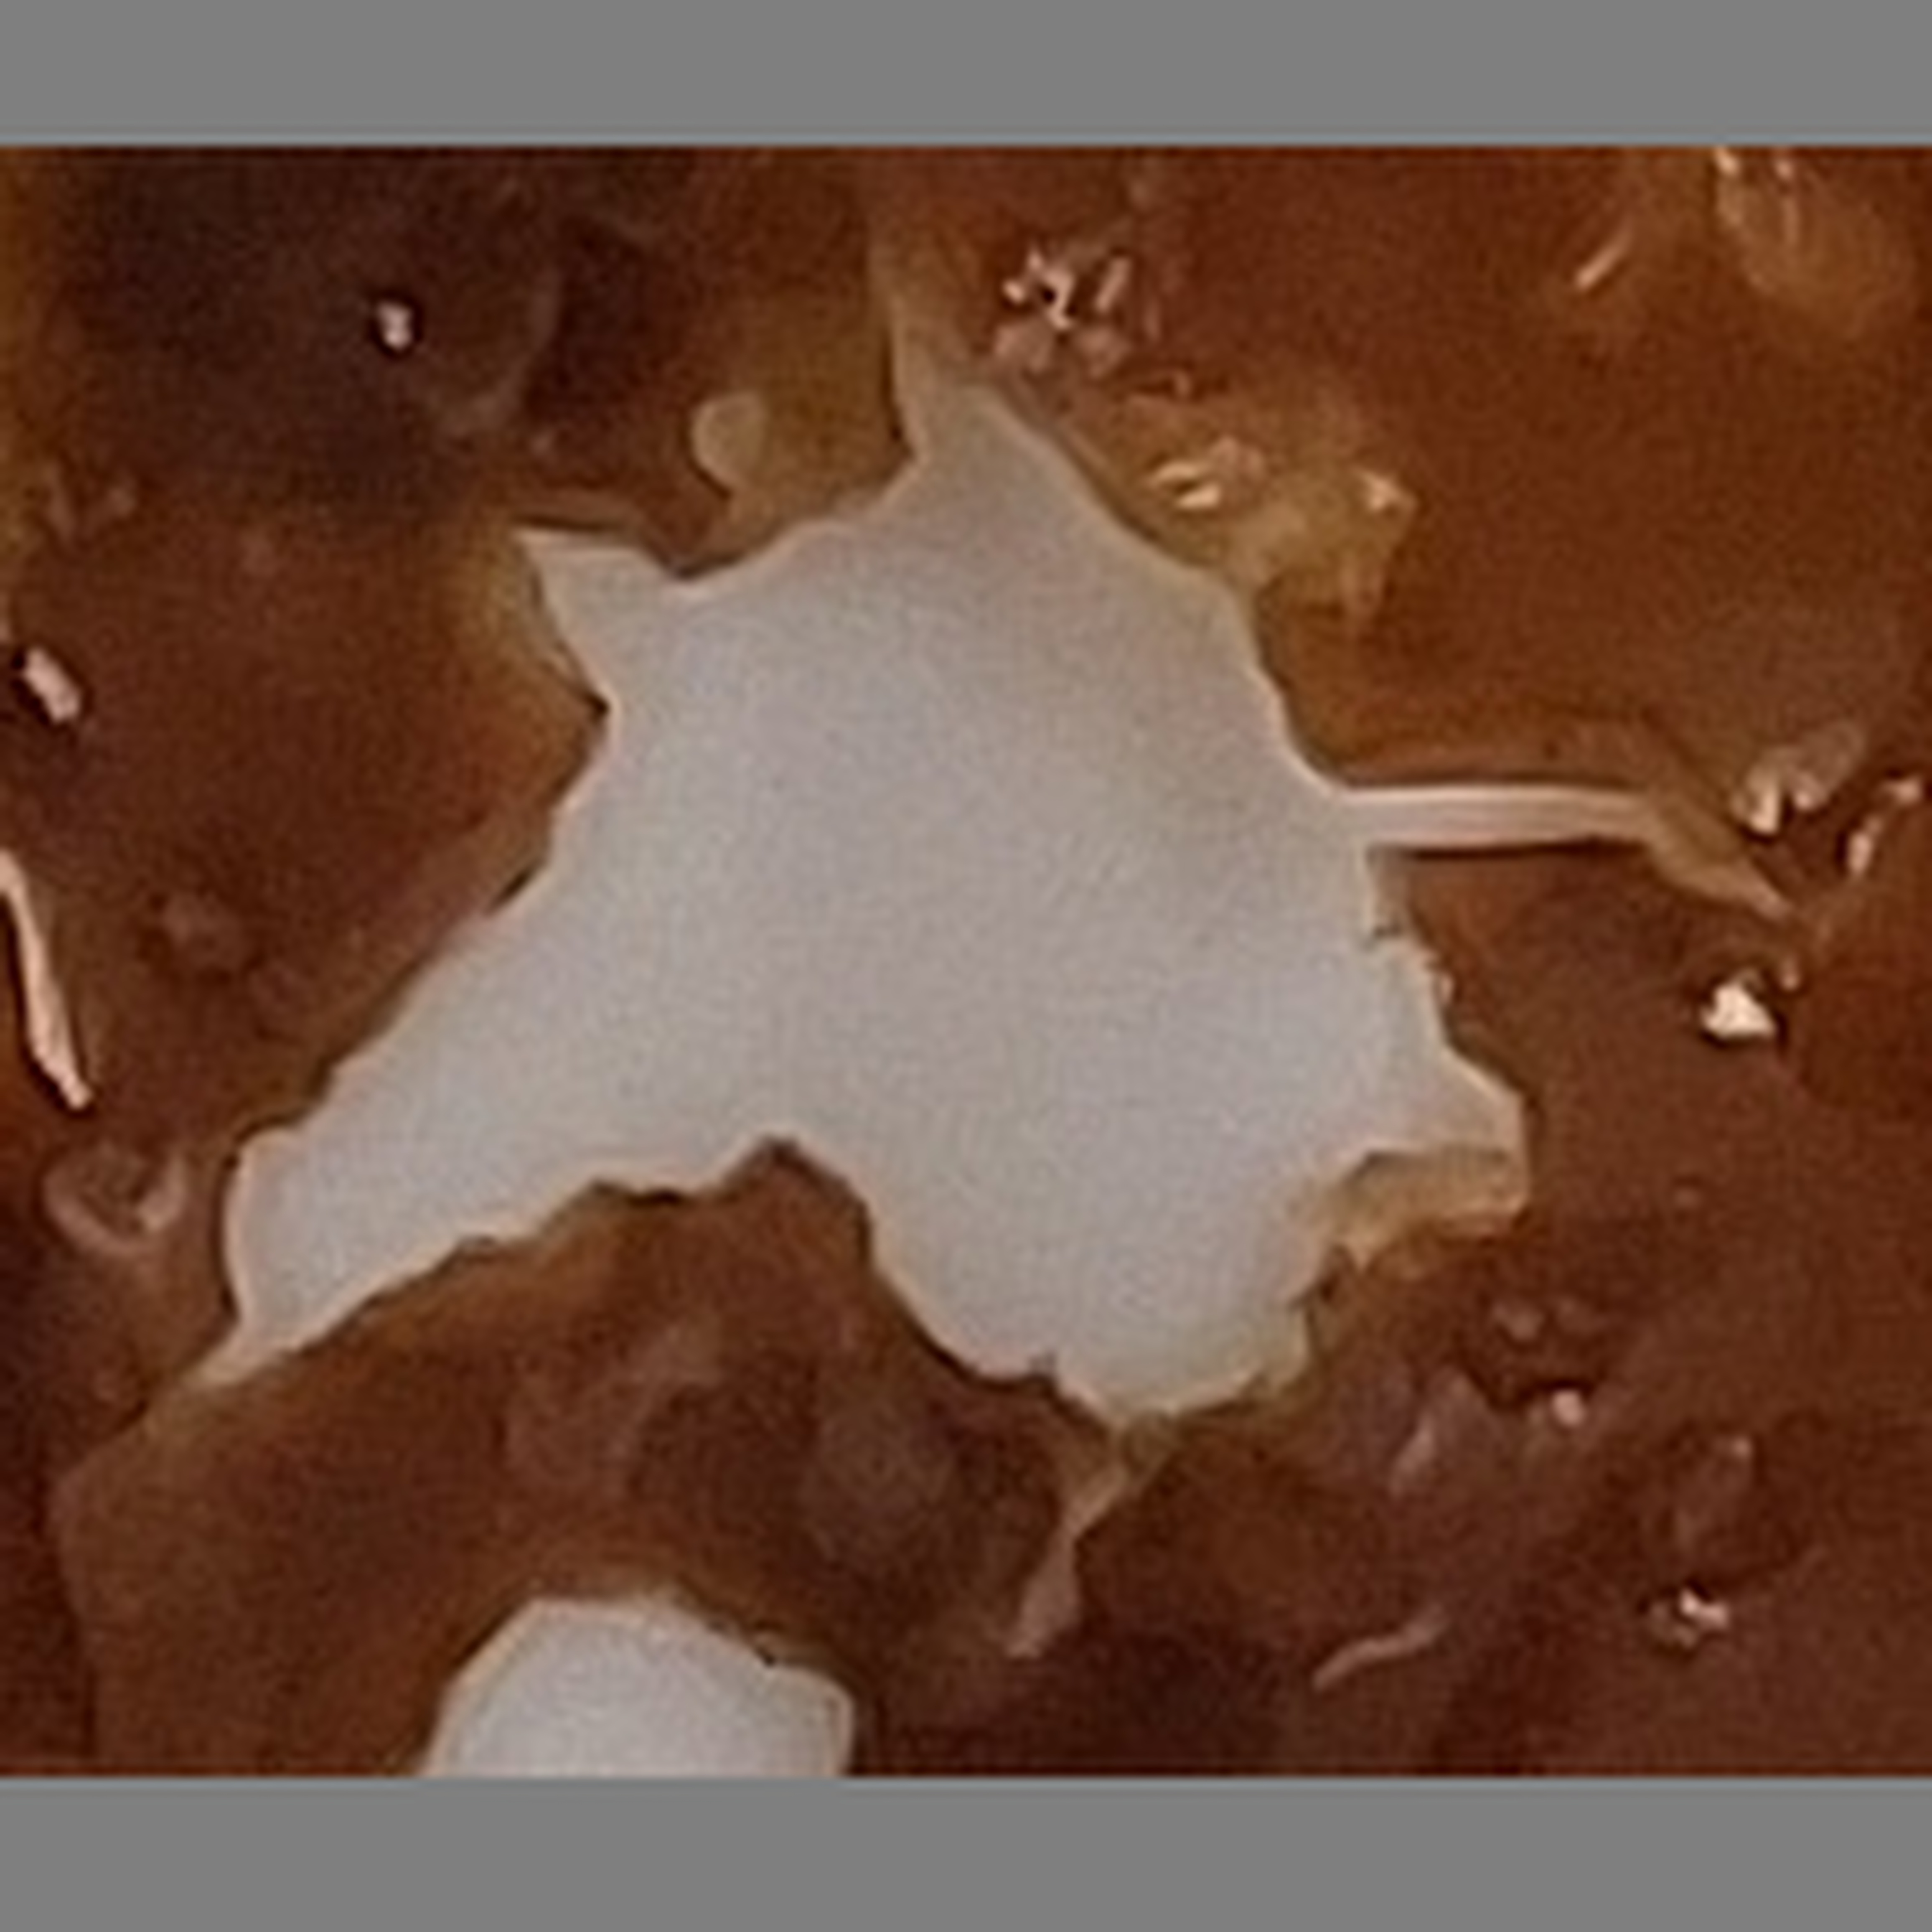
\includegraphics[width=\linewidth]{imaxes/mal_recorte_4.jpg}
        \caption{Burato interior en alga recortado como a propia alga.}
    \end{subfigure}

    \vspace{0.15em}

    \begin{subfigure}[t]{0.42\textwidth}
    \centering
    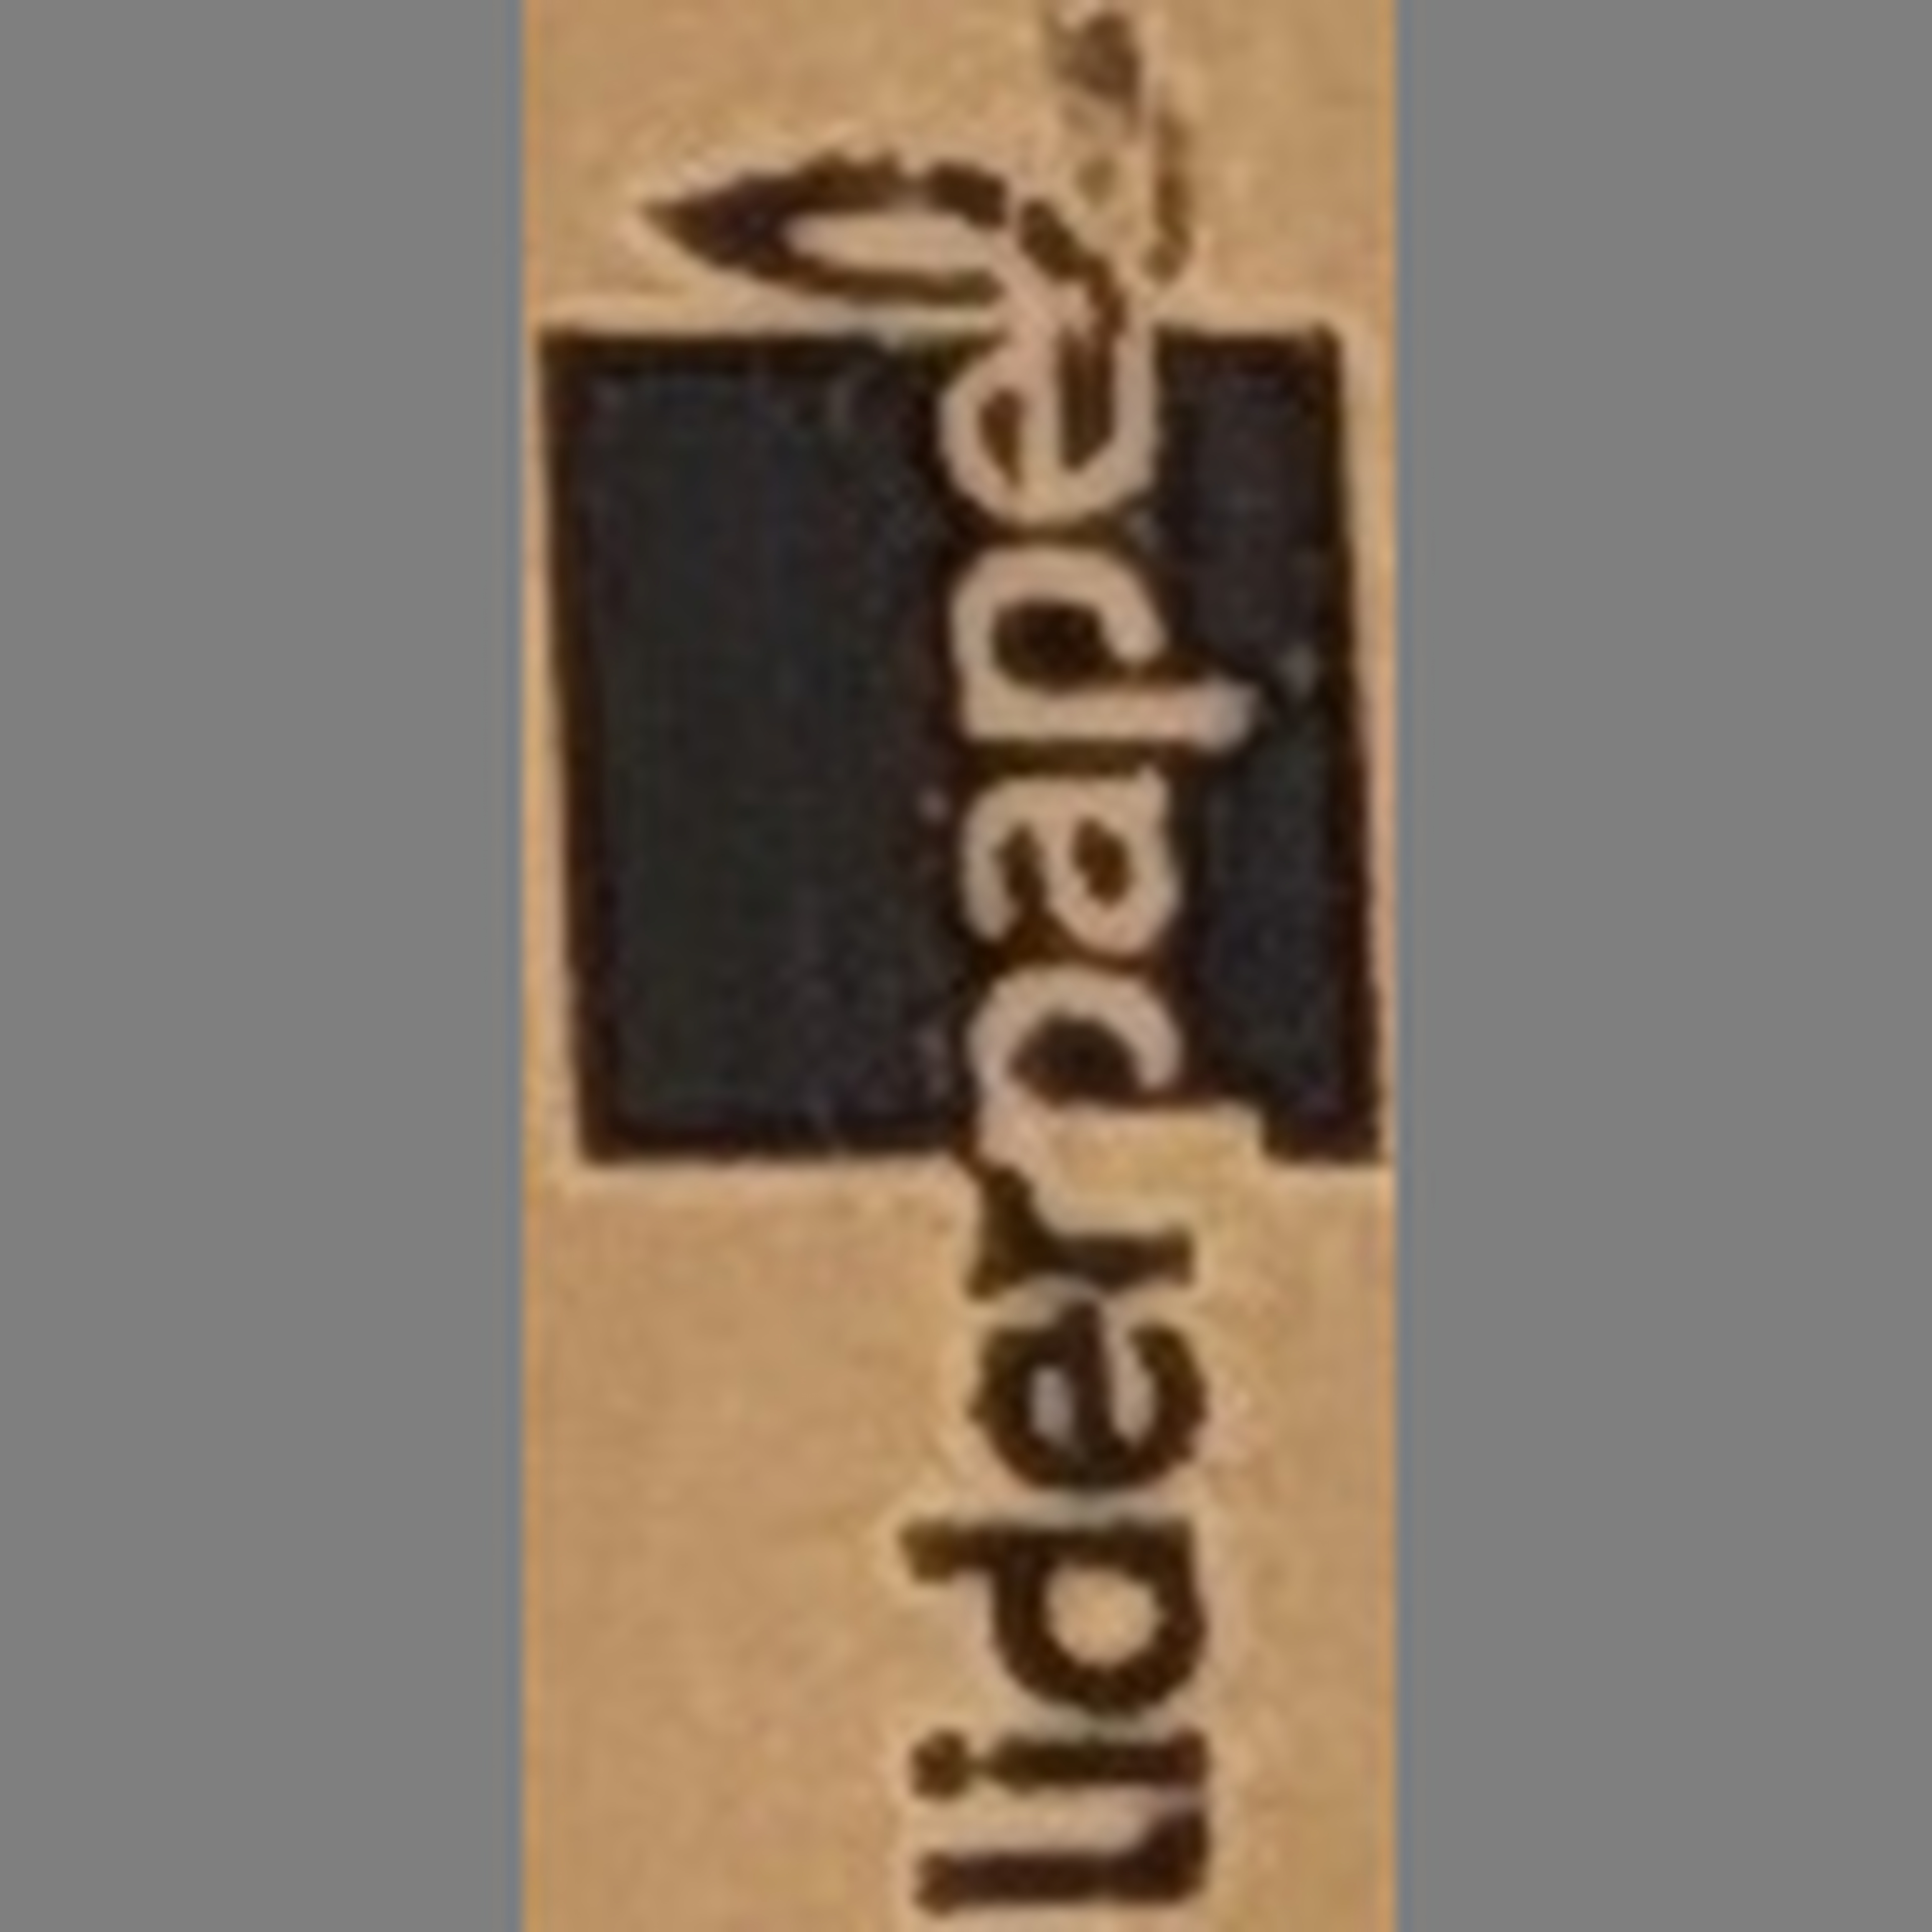
\includegraphics[width=\linewidth]{imaxes/mal_recorte_5.jpg}
    \caption{Logo de regra recortado como alga.}
    \end{subfigure}
    \caption{Exemplos de recortes erróneos na primeira iteración de procesado do dataset.}
    \label{fig:recortes-erroneos}
\end{figure}

\subsection{Segunda Aproximación}
\subsubsection{Preparación do \textit{dataset}}
Unha vez resultaron evidentes as limitacións da primeira aproximación, decidiuse buscar un método
máis robusto fronte á elevada variabilidade do \textit{dataset}. A alternativa escollida foi
empregar \gls{yolo}, aproveitando a súa capacidade para a detección de obxectos en condicións máis
heteroxéneas ca as que podían abordarse con regras clásicas de visión por computador.

A principal dificultade inicial deste cambio de enfoque non residía tanto no modelo en si como na
preparación dun conxunto de adestramento axeitado. Para iso implementouse un novo \textit{script} de
Python, denominado \texttt{04\_recortar\_yolo.py}, orientado a xerar imaxes e anotacións nun formato
compatible co adestramento de YOLO.

Este \textit{script} reutilizaba a lóxica desenvolvida na primeira aproximación para propor,
automaticamente, un \textit{bounding box} candidato para a alga presente en cada imaxe. Dado que esta
detección inicial non resultaba suficientemente fiable, incorporouse un modo adicional mediante o
\textit{flag} \texttt{--review}, que abría unha interface gráfica sinxela para revisar manualmente os
recortes propostos. Nesta interface, que se mostra na Figura~\ref{fig:gui-recortes-manuais}, visualizábase
a imaxe orixinal xunto coa \textit{bounding box} xerada automaticamente e decidíase se
debía aceptarse ou descartarse.

Os controis da interface mantivéronse deliberadamente simples para non dificultar o proceso de
revisión: \texttt{ESC} ou \texttt{q} para saír, \texttt{Enter} para aceptar o recorte e calquera outra
tecla para descartalo. Deste xeito foi posible realizar unha curación manual dos candidatos xerados
pola primeira aproximación e construír un conxunto de mostras válidas para a detección dunha única
clase, definida como \texttt{CLASS\_ID=0} e \texttt{CLASS\_NAME='alga'}.

Ademais da revisión manual, o \textit{script} xeraba automaticamente a estrutura de directorios
requirida por YOLO, separando imaxes e etiquetas nos subdirectorios correspondentes a
\textit{train} e \textit{val}. Así mesmo, convertía o formato das caixas delimitadoras ao esquema
normalizado empregado por YOLO, isto é, \texttt{(x\_center, y\_center, width, height)}. A división
entre ambos os dous subconxuntos realizábase de maneira aleatoria segundo a proporción indicada polo
\textit{flag} \texttt{--val-split}. Xunto con estas saídas, xerábase tamén un ficheiro
\texttt{data.yaml} coa información básica da clase necesaria para iniciar o adestramento do modelo.

\begin{figure}[htbp]
    \centering
    \begin{subfigure}[t]{0.65\textwidth}
        \centering
        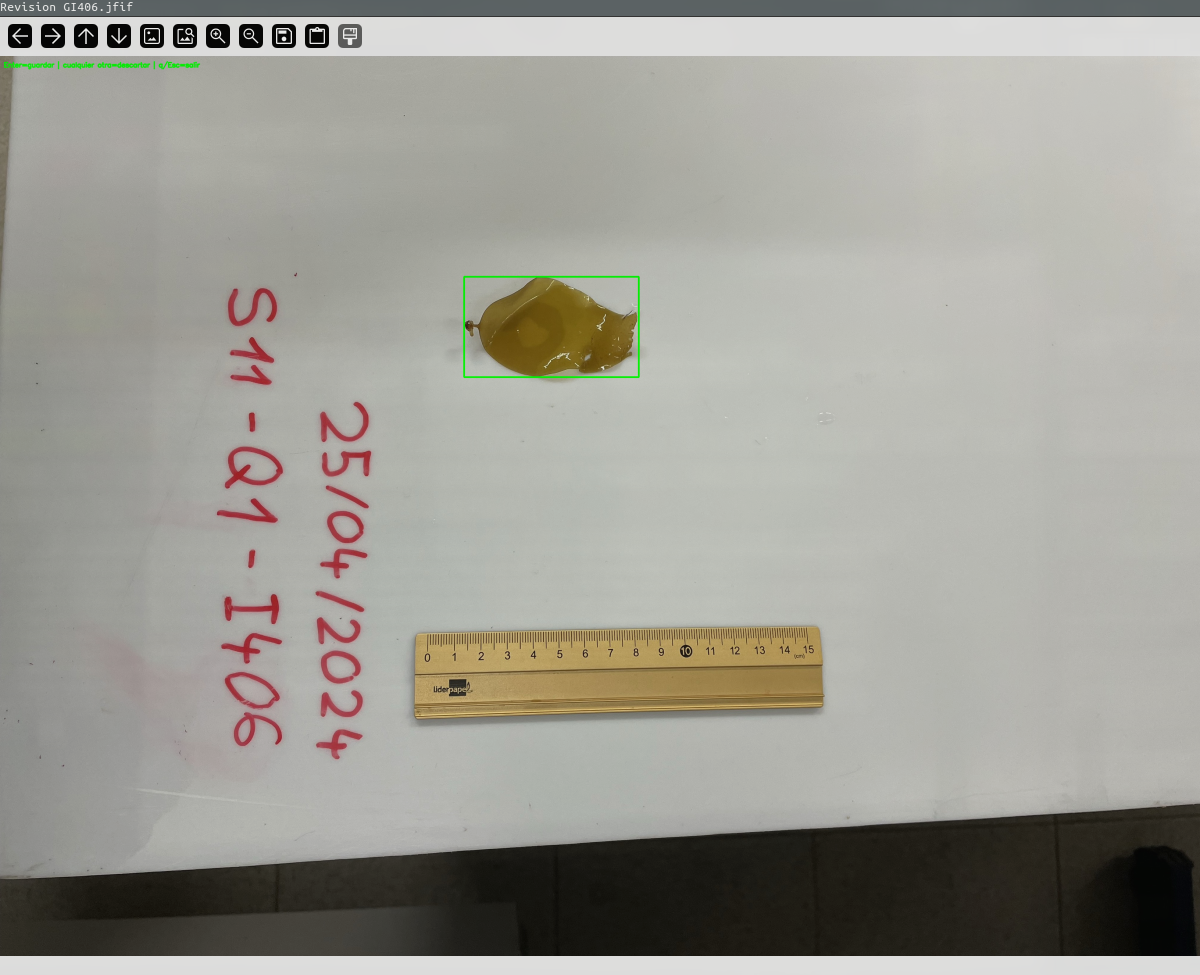
\includegraphics[width=\linewidth]{imaxes/gui_recorte_correcto.png}
        \caption{Interface do script cun recorte correcto, aceptaríase manualmente.}
    \end{subfigure}

    \vspace{0.6em}

    \begin{subfigure}[t]{0.65\textwidth}
        \centering
        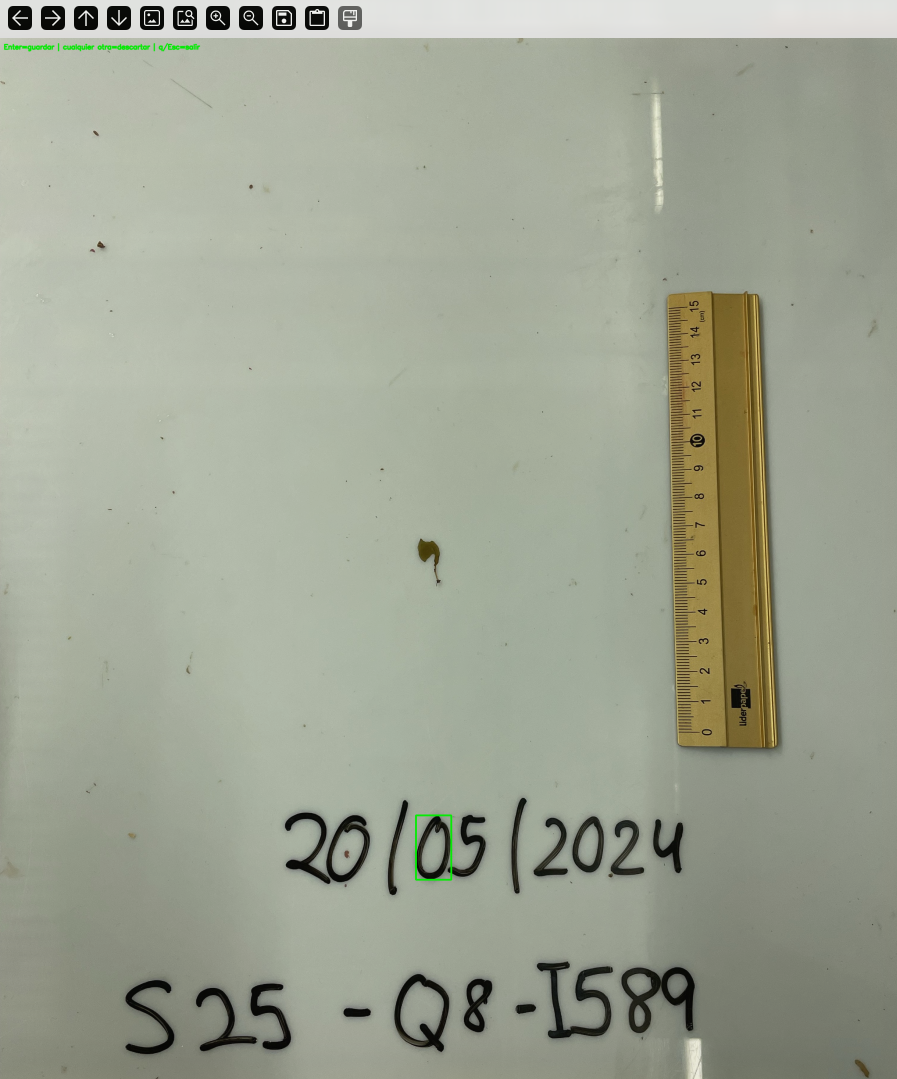
\includegraphics[width=\linewidth]{imaxes/gui_recorte_erroneo.png}
        \caption{Interface do script cun recorte erróneo, rechazaríase manualmente.}
    \end{subfigure}
    \caption{Exemplos da interface para decidir se usar ou non o recorte automático no dataset.}
    \label{fig:gui-recortes-manuais}
\end{figure}

Mediante este procedemento obtívose finalmente un conxunto de datos anotado de maneira suficientemente
consistente para iniciar os experimentos con YOLO. A revisión manual resultou necesaria precisamente
porque os recortes propostos pola primeira aproximación seguían presentando erros frecuentes, o que
impedía a xeración automática dun conxunto fiable.

Despois de revisar manualmente arredor de 1300 imaxes, obtívose un \textit{split} final composto por
636 imaxes de \textit{train} e 146 de validación, correspondentes a unha partición aproximada do
80\,\% e 20\,\%, respectivamente. Aínda que este volume era reducido en relación co tamaño total do
\textit{dataset}, considerouse suficiente como punto de partida para o adestramento dun detector
orientado á localización dunha única clase.


\subsubsection{Adestramento de YOLO}

\section{Normalización de imaxes de algas}
\textcolor{red}{\textbf{TODO: Detallar o proceso de recorte, limpeza e normalización das imaxes antes
da súa entrada ao modelo de inferencia.}}

\section{Arquitectura e adestramento da CNN}
\textcolor{red}{\textbf{TODO: Describir a arquitectura empregada, o procedemento de adestramento e os
criterios seguidos para avaliar o modelo.}}

\section{Integración da pipeline}
\textcolor{red}{\textbf{TODO: Explicar como se integraron os distintos compoñentes nunha ferramenta
usable polos expertos.}}
